\documentclass{article}
\usepackage{amssymb, amsmath}
\usepackage{anysize}
\usepackage{graphicx}
\marginsize{2cm}{2cm}{2cm}{2cm}
\newcommand{\bs}[1]{\boldsymbol{#1}}
\begin{document}
Started 10/3 2013 or somewhere around there.


\textbf{HughesLiuZimmermann1981}
\begin{itemize}
\item Material domain in motion??.
\item Try to understand examples better.
\end{itemize}

\textbf{BraessWriggers2000}
\begin{itemize}
\item Free surface flow as an example of the ALE method permitting a good mesh (no distortion) and an accurate description of boundaries at the same time (due to Eulerian description being used horizontally and Lagrangian description vertically).
\item I should emphasize that the convective velocity isn't physical!
\item Aspect ratio of elements as r\_out/r\_in.
\item (p.103) In case of Lagrangian description: mesh distortion a problem, but can be solved using remeshing. Computationally costly though, and a source of discretization errors.
\item Remeshing is used.
\end{itemize}

\textbf{FrancaFarhat1995}
\begin{itemize}
\item Stabilization operator
\[P(v) = -\sigma v + a\nabla v + \kappa\Delta v\]
instead of
\[P(v) = \sigma v + a\nabla v + \kappa\Delta v\]
\end{itemize}

\textbf{BankWelfert1990}
\begin{itemize}
\item 
\end{itemize}

\textbf{Stromberg2011}
\begin{itemize}
\item Uses decoupled thermomechanical equations.
\item Doesn't seem to model heat exchange with environment.
\item Coded in Fortran? Not clear.
\item Global sliding assumed!
\item S-U-stabilization implemented.
\item Why call the kinematical model "Eulerian"? Due to no translation of wheel? (Then, no linear acceleration effects?)
\item No problems with energy dissipation?
\item Only wheel--brake block contact. No translation.
\end{itemize}

\textbf{PaukYevtushenko1997}
\begin{itemize}
\item Sliding using an Eulerian approach.
\item The effect of rail chill shown (more prominent for higher Pe).
\end{itemize}

\textbf{WauerSchweizer2010}
\begin{itemize}
\item Many good thermoelasticity-references in the beginning.
\item Eulerian disc-brakeblock-model (as in Stromberg2011) \emph{using cylindrical coordinates}.
\item No mention of numerical instability or measures to mitigate it, probably because there is none, due to the use of cyl. coords.
\item Insight: If \emph{any} convection, then not Lagrangian description. If \emph{any} movement of nodes, then not Eulerian description. Therefore ALE.
\end{itemize}

\textbf{SchweizerWauer2001}
\begin{itemize}
\item Very nice introduction, discussing thermomechanical coupling.
\item Metals -- polychrystalline. Rubber -- polymeric.
\end{itemize}

\textbf{Galantucci1999}
\begin{itemize}
\item Lagrangian formulation of hot rolling ($>$800 deg used). Rolling 2$\pi$/4 and 2$\pi$.
\end{itemize}

\textbf{Belytschko1980}
\begin{itemize}
\item FSI application with ALE (called quasi-Eulerian here).
\end{itemize}

\textbf{Hughes1995}
\begin{itemize}
\item Stabilized methods originate from a particular class of subgrid scale methods.
\item $\tau$ can be defined exactly: it can be derived from first principles.
\item Check Hughes publications following this paper.
\item Bubbles identified as approximations of element Green's functions.
\item Bubbles in the subgrid + static condensation $\approx$ subgrid scale model + assumption of subgrid contribution vanishing on element boundaries.
\item Expression for $\tau$ derived, involves $g(x,y)$.
\end{itemize}

\textbf{AmsdenHirt1973book}
\begin{itemize}
\item Mostly describes the code YAQUI (which uses finite differences).
\item Other techniques L/E/ALE mentioned, e.g. ICE (?).
\item I should check out reference 2 (HirtAmsdenCook1997), it describes the ALE technique in detail.
\end{itemize}

\textbf{HirtAmsdenCook1997}
\begin{itemize}
\item A very simple ALE description seems to be used. It seems to be described in terms of moving mesh points rather than some formulation preceding discretization based on continuum mechanics.
\item Each time step involves 3 phases, the last of which is optional re-zoning: moving vertices to keep a good mesh quality and thereby causing convection. An upwind averaging scheme is here used to avoid numerical instability (p. 209).
\item The method seems so closely tied to the mesh and the practical computational algorithm. They don't start from first principles (continuum mechanics) as for instance Donea \& Huerta, Nackenhorst etc.
\end{itemize}

\textbf{FrancaFarhat1994}
\begin{itemize}
\item In a pure diffusion prolem, the node values at the nodes included in the linear mesh are the same whether linear or quadratic interpolation is used.
\item I'm wondering what the 1D example has to do with bubbles. It seems that linear--quadratic is what's compared, rather than bubbles on/off.
\item But int he 2D example, they use an approximation consisting of a linear interpolation + a higher order bubble (for which they need to introduce an extra node).
\end{itemize}

\textbf{FrancaFrey1992}
\begin{itemize}
\item Compares a stabilization method by Douglas--Wang with the GLS method for Stokes flow.
\item Hints that the pure least-squares method gives too dissipative results for the advection--diffusion equation.
\item Example: 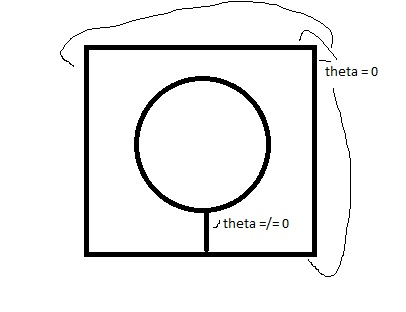
\includegraphics[width=3cm]{figures/FrancaFrey1992_img1.jpg}
\item Example: 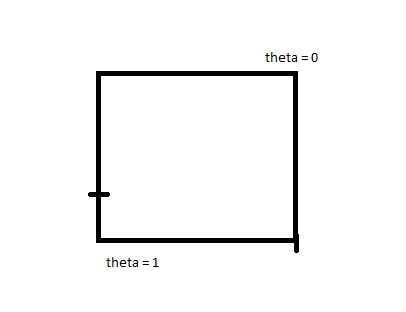
\includegraphics[width=3cm]{figures/FrancaFrey1992_img2.jpg}. Here, quad is considerably better than lin for equal number of dofs.
\item Some development in the chocie of $\tau$.
\end{itemize}

\textbf{BurmanHansbo2004}
\begin{itemize}
\item Term added to the weak form penalizing gradient jumps across element boundaries.
\item It is said that the source of the added stability is the fact that the edge of operator controls the projection error of the term $\bs{\beta}\cdot\nabla v$ $(\bs{a}\cdot\nabla\theta)$ in the case of convection--diffusion.
\item Some error estimates are given and proven.
\item Something called "shock capturing" is mentioned, which was used in a previous paper. The numerical examples both do and don't use shock capturing.
\end{itemize}

\textbf{GaoHuang2006}
\begin{itemize}
\item Insightful introduction about:
\begin{itemize}
\item Disc brakes, pros and failure modes, including thermomechanical effects.
\item How fatigue cracks initiate and spread.
\item Comment on the assumption of a constant sliding velocity in braking simulations.
\end{itemize}
\item Disc braking model with variable speed (down to 0).
\item The model used uses simplifying geometrical and thermal assumptions that make it very specific to the given application.
\item FEM using ANSYS.
\item On hot spots and how their related temperature spikes can be avoided.
\item Results show fluctuating temperatures and stresses. Up due to frictional heat generation and down due to dissipation/convection. (I don't really understand) when studied point if outside of the contact region (the part in parenthesis above was strikethrough:ed, I don't know what I meant by that). One cycle per revolution.
\item Unclear whether Eulerian or Lagrangian description.
\item Contact model unclear.
\end{itemize}


\textbf{HuertaLiu1988}
\begin{itemize}
\item History of ALE (just as in DoneaHuerta2003book).
\item Spurious oscillations when Galerkin method is used for convection--dominated problems is because the FE equations are not self-adjoint.
\item "The [ALE] reference frame is fixed, but its movement [...] is arbitrary...". If this isn't a contradiction, then what does "fixed" mean in this context?
\item Tsunami, dam-break and sloshing problem considered. Large free-surface motion.
\item The use "a SUPG method for the mesh updating equation". What does this mean?
\item Kinematical description different for each problem, but in general Eulerian in the horizontal direction and Lagrangian in the vertical direction.
\end{itemize}


\textbf{Baiocchi1993}
\begin{itemize}
\item Intro mentions bubbles + static condensation (SC) viewed as the addition of a stabilizing term to the FE problem.
\item Addition of bubbles + SC formulated in abstract form. The resulting stabilization term added to the RHS is derived for the general case...
\item ...and then for two specific examples, one of which is the advection--diffusion problem.
\item If bubble functions + SC is equivalent to the SUPG among others, why does it work better in the rotating disc case? Because the space used for the bubble functions is of a particularly high quality?
\item Paper establishes "a rather general link between two major families of stabilizing techniques". For the first time I guess? Nice.
\end{itemize}

\textbf{BrezziBristeau1992}
\begin{itemize}
\item Similar to Baiocchi1993 (Brezzi \& Franca authors on both). The equivalence between Galerkin + bubbles and stabilized FE methods is established. The limit $\kappa \rightarrow 0$ is investigated.
\item The stability of different methods are investigated quantitatively.
\item Relationship between bubbles and SUPG was first noted in Rogé's thesis (so, I should cite that if I write about it).
\end{itemize}

\textbf{XuJiang2001}
\begin{itemize}
\item Introduction:
\begin{itemize}
\item On rolling contact, where it happens and associated problems (damage phenomena).
\end{itemize}
\end{itemize}

%\textbf{key}
%\begin{itemize}
%\item item
%\end{itemize}






\textbf{WriggersMiehe1994}

\begin{itemize}
\item The paper presents a microgeometrical contact interface model for thermomechanical frictional contact.
\item Contact geometry described in detail.
\item Sophisticated interface laws for normal contact stress and contact heat flux given. Seems like no mention of frictional heat generation? Slip is split into an elastic part and a plastic part.
\item "The resistance agains heat transfer is mainly due to the low percentage of physical surface area which is really in contact."
\item Thermoelasticity constitutive response assumed.
\item Gough--Joule coupling effect included (no mention about neglecting it).
\item A staggered scheme (problem split into "a purely mechanical subproblem (M) at frozen temperature" (called a "predictor") and "a purely thermal subproblem (T) at frozen configuration (called a "corrector")). The algorithm is said to be identical to the one suggested in Argyris and Doltsinis [16].
\item Numerical examples provided. Most of them feature a thermoelastic body pressed against a rigid but heat-conducting body. Idealized thermal isolation or fixed temperatures are assumed at surfaces.
\end{itemize}











\textbf{ZiefleNackenhorst2007}
\begin{itemize}
\item Introduction:
\begin{itemize}
\item So Oden and Lin and Padovan (and Zeid I guess) are the first examples of FEM being used for rolling contact. They used a relative kinematics approach or whatever it's called. (I guess it is impossible to model rolling contact using FEM using a purely Lagrangian description.) ALE is more general though.
\item "[...] the history of particles which initially got into contact has to be traced to evaluate the friction law". Why? Aren't slip velocities enough? "A common procedure [regarding treatment of frictional contact within an ALE context] is the penalization of the slip velocities which are computed directy within the relative kinematic framwork". Is that what I'm doing?. "A further complication arises from the fact that by this approach the tangential contact traction is not computed directly from a constitutive law". I don't understand this, I thought that was what I was doing.
\end{itemize}
\item The slip distances can be computed from the slip velocities by temporal integration, which can be exchanged for spatial integration due to the fact that time derivatives are exchanged for spatial derivatives in the convective description (is this true for the transient case as well?)
\item Slip distances introduced as extra variables.
\item "Once [the slip distribution has been obtained], the standard concepts for the treatment of frictional contact problems can be used, see eg. [18] [a paper by Wriggers].". Why is the slip distance (undifferentiated) needed in a friction law? How is "slip distance = 0" a valid stick condition?
\end{itemize}

\textbf{ZiefleNackenhorst2007\_2}
\begin{itemize}
\item Introduction:
\begin{itemize}
\item "First approaches on the numerical treatment of rolling contact by finite element methods based on rather simple relative kinematic formulations...". Reference given to Oden and Lin.
\item Check out reference 6 (Faria et. al.). I supposed to mention ALE (but I don't find any explicit reference to it, not by that name anyway).
\item Claims that ABAQUS can handle treatment of inelastic material parameters in an ALE-context. I didn't find anything on this though. Perhaps they call it something other than ALE.
\item "No sound mathematical basis for the treatment of inelastic material properties within the ALE-framework is available so far, which for example enables for error estimation based on computed results. This contribution is aimed to close these gaps".
\end{itemize}
\item Insight: I should know the physical interpretation of all my terms.
\item An additional update procedure for the internal variables has to be provided. This requires tracing the material particles as they move through the fixed FE mesh. This problem is well known in fluid mechanics. 
\item Insight from the above: Any advection-related problem of the ALE approach can probably be found (as well as its solution) in fluid mechanics.
\item In the ALE context, time derivatives in the advection equation are replaced by spatial derivatives (at least in the stationary case).
\item Perhaps "convection": the mathematical concept and "advection": specifically referring to the transport of physical quantities.
\item The "advection equation" is solved to update the internal variables.
\item Different numerical schemes and associated stabilization methods are compared. This is said: "The upstream method is stable, but suffers strongly under diffusion effects". I'm wondering if these are the same as those we observe in paper 2. Perhaps not, since this is 1D.
\item Overshoot-effects result from differences between inflow and the outflow within one element.
\item A fractional-step method (a staggered approach) is used to incorporate the solution of the advection equation in the FE-problem: 1. Solve nonlinear ALE rolling contact problem. 2. Smooth out internal variables for a  $C^0$-smooth representation. 3. Solution of the advection problem by TDG-schema.
\item Question regarding part 2 above: Isn't information lost as the internal variable data is smoothed out in coarser regions of the mesh?
\item As material particles are convected through the contact region, the contact pressure distribution becomes asymmetric for medium convective velocities: for high conv. vel.: no relaxation, for low conv. vel.: total relaxation.
\item One disadvantage of the ALE approach is additional computational effort when inelastic material properties have to be taken into account.
\end{itemize}

\textbf{ZiefleNackenhorst2008}
\begin{itemize}
\item Seems like a combination of the last two papers.
\item Introduction:
\begin{itemize}
\item ALE methods have been developed rapidly in other fields of engineering application, i.e. FSI and metal forming processes (see review paper [13]).
\item Traditional engineering approaches to treatment of inelastic material properties involves integrating the history along predefined rings of integration points (e.g. Faria, Oden/Lin). However, this poses a problem with unstructured meshes and isn't built upon a sound mathematical basis. Le Tallec and Rahier [22] represents a first step towards something more mathematically sound.
\end{itemize}
\item Insight: I should include the expression for $\boldsymbol{v}$ as well and discuss terms such as "guiding velocity" and actual convective velocity.
\item "the accurate and efficient numerical solution of advection equations is still part of the current research in the field of computational fluid dynamics". Implying that ALE approaches can benefit from this research as well.
\item "The TDG approach uses a coupled space-time-discretization instead of the common concept of semi-discretization" apparently.
\item The smoothing out of the internal variables is said to be performed using a "super-convergent patch recovery technique".
\item Regarding Figure 7 of the rolling kinematics. Isn't this a very idealized picture? Is it actually used?
\item "The asymmetric of the contact pressure distribution in the mid-frequency range results in a torque which contributes to the rolling resistance."
\item He uses the slip
\[S = \frac{V_T-V_C}{VT}\]
while I use
\[S = 2\frac{V_T-V_C}{VT+V_C}\]
\item "If inelastic material properties are applied to the model, the computation time increases significantly". I'm wondering: How big is the increase in computational effort in the \emph{Lagrangian} case when inelastic material props are applied?
\item "An explicit scheme has been suggested for the computation of rolling contact problems of inelastic bodies, known as \emph{Fractional-Step}-method from other established ALE-applications, because a fully implicit algorithm seems to be not computable for real life problems yet." Because of excessive computational effort, or what? So the use of the fractional-step method is by necessity rather than by choice?
\item "concerning the frictional rolling contact problem a novel and fully implicit approach for the treatment of tractive rolling contact within the ALE framework for steady-state rolling has been presented". What does "implicit" mean? Requiring iterations?
\item Ref [10] seems to be another good summary paper on ALE methods (by Donea et. al.).
\end{itemize}

\textbf{BrinkmeierNackenhorst2009}
\begin{itemize}
\item Paper focuses on "the transient dynamics response with respect to rolling noise prediction". A modal analysis will be used. The transient response due to excitation from different road surface textures will be investigated next.
\item Quite applied, a little bit outside my area of interest.
\end{itemize}

\textbf{Suwannachit2013}
\begin{itemize}
\item Paper is about thermomechanical analysis of stationary rolling tires using the ALE approach. Large deformations are implemented along with a thermoviscoelastic constitutive model including internal dissipation.
\item Introduction:
\begin{itemize}
\item Internal dissipation is well known to be the main source of temperature rise in tires.
\item "The coupled momentum and energy balance equations are solved with an isentropic operator-split scheme".
\item The transport of inelastic variables during rolling is solved using the TDG method as described in ref. [26].
\end{itemize}
\item Constitutive parameters are temperature-dependent.
\item Viscous hysteresis decreases with increasing environmental temperature and even vanishes eventually. This is captured by their model.
\item They don't want to solve the balance eqs. simultaneously, because the tangent operator is "large" and "nonsymmetrical" in that case. They use a staggered (fractional-step) approach. They here choose the isentropic operator-split method over the isothermal method because the former is unconditionally stable.
\item Frictionless contact considered (and frictional heating is as a consequence not considered) "in order to focus on the heat generation caused by inelastic constitutive behaviour".
\item On the TDG approach: "The major advantage of this approach is its control over numerical inaccuracies, like diffusion and oscillation".
\item "although the global representation of balance equations is time-independent for stationary rolling, integration in time is still needed for the evolution of inelastic strains." A staggered computational scheme is used: i) mechanical subproblem. ii) nonlinear heat conduction, iii) transportation of internal variables.
\item The Gough--Joule effect is neglected (both the thermoelastic and the thermoviscoelastic part of it).
\item For a clear observation of the hysteretic heating, the heat transfer with environmental air is neglected. (perhaps I should have motivated my neglection of this effect better as well).
\item Cool simulation: first inflation (statically), then setting the wheel into rotation, then bringing it into contact with the surface. I guess all this is done "statically" and not transiently.
\item Consistent linearization is employed and quadratic convergence rate of both mech. and therm. subproblems are achieved (using Newton-Raphson iterations).
\item "In our numerical studies, the stationary rolling state was obtained within only few revolutions". I don't get this, isn't everything stationary?
\end{itemize}

\end{document}

%\textbf{key}
%\begin{itemize}
%\item Introduction:
%\begin{itemize}
%\item item
%\end{itemize}
%\item item
%\end{itemize}